% Twentyfold Way
\section{Distributions: The Twentyfold Way}
\label{twentyfoldway}

These notes (in particular) need review. There is a deeper perspective on distributions that is constructed in terms of functions and equivalence classes, which is poorly developed here so far, and I think there are some errors too. The different "interpretations" are also not well-developed here.

The twentyfold way is a taxonomy of distribution problems developed by Kenneth Bogard in his book \textit{Combinatorics through Guided Discovery} \cite{bogart2004combinatorics}. It divides up the way in which $k$ objects may be assigned to $n$ individuals, subject to whether the objects are distinct or identical, and subject to conditions on how the objects are received.


\begin{quote}
\textit{When we are passing out objects to recipients, we may think of the objects as being either identical or distinct. We may also think of the recipients as being either identical (as in the case of putting fruit into plastic bags in the grocery store) or distinct (as in the case of passing fruit out to children). We may restrict the distributions to those that give at least one object to each recipient, or those that give exactly one object to each recipient, or those that give at most one object to each recipient, or we may have no such restrictions. If the objects are distinct, it may be that the order in which the objects are received is relevant (think about putting books onto the shelves in a bookcase) or that the order in which the objects are received is irrelevant (think about dropping a handful of candy into a child’s trick or treat bag). If we ignore the possibility that the order in which objects are received matters, we have created $2\times2\times4 = 16$ distribution problems. In the cases where a recipient can receive more than one distinct object, we also have four more problems when the order objects are received matters. Thus we have 20 possible distribution problems.} - Bogart, \textit{Combinatorics Though Guided Discovery}, Chapter 3.
\end{quote}


What I like about this approach is that the challenge with most of the basic combinatorics problems is to figure out the right way of counting. For this reason, the idea of having a unified handbook-like taxonomy is very appealing. The weakness (in my opinion) is that the language of "objects" and "recipients" is unclear because in practice it's not obvious which is which: if there are $k$ students and $n$ teachers, do the teachers receive students, or do the students receive a teacher? 

A way to resolve this is to say that an object can have only one recipient, but that a recipient might receive more than one object. A more formal path is to think of the act of creating combinations in terms of functions. 

\begin{itemize}
\item The elements of the domain are the objects. 
\item The elements of the range are the recipients. 
\item A function can be many-to-one, but it should not be one-to-many. 
\end{itemize}

\subparagraph{Favorite Teachers} At a school with $k$ students and $n$ teachers, the students all have a favorite teacher. (They might all like the same one.). How many ways are there for all of the $k$ students to pick a favorite? 

\textit{Objects:} $k$ students. \textit{Recipients:} $n$ teachers. Many students might have one favorite teacher. There are $n^k$ combinations. 

\subparagraph{Assembling a Team} Out of a choice of $n$ athletes, a coach must assemble a team of $k$. How many ways are there to form a team? 

\textit{Objects:} n athletes. \textit{Recipients:} team, not on the team. Many athletes can be assigned to one outcome of being on the team or not being on the team. There are ${n \choose k}$ combinations for the team, which is the same number as the ${n \choose n-k}$ selections for the bench. 



\begin{figure}
  \caption{Bogart's Twentyfold Way}
  \centering
    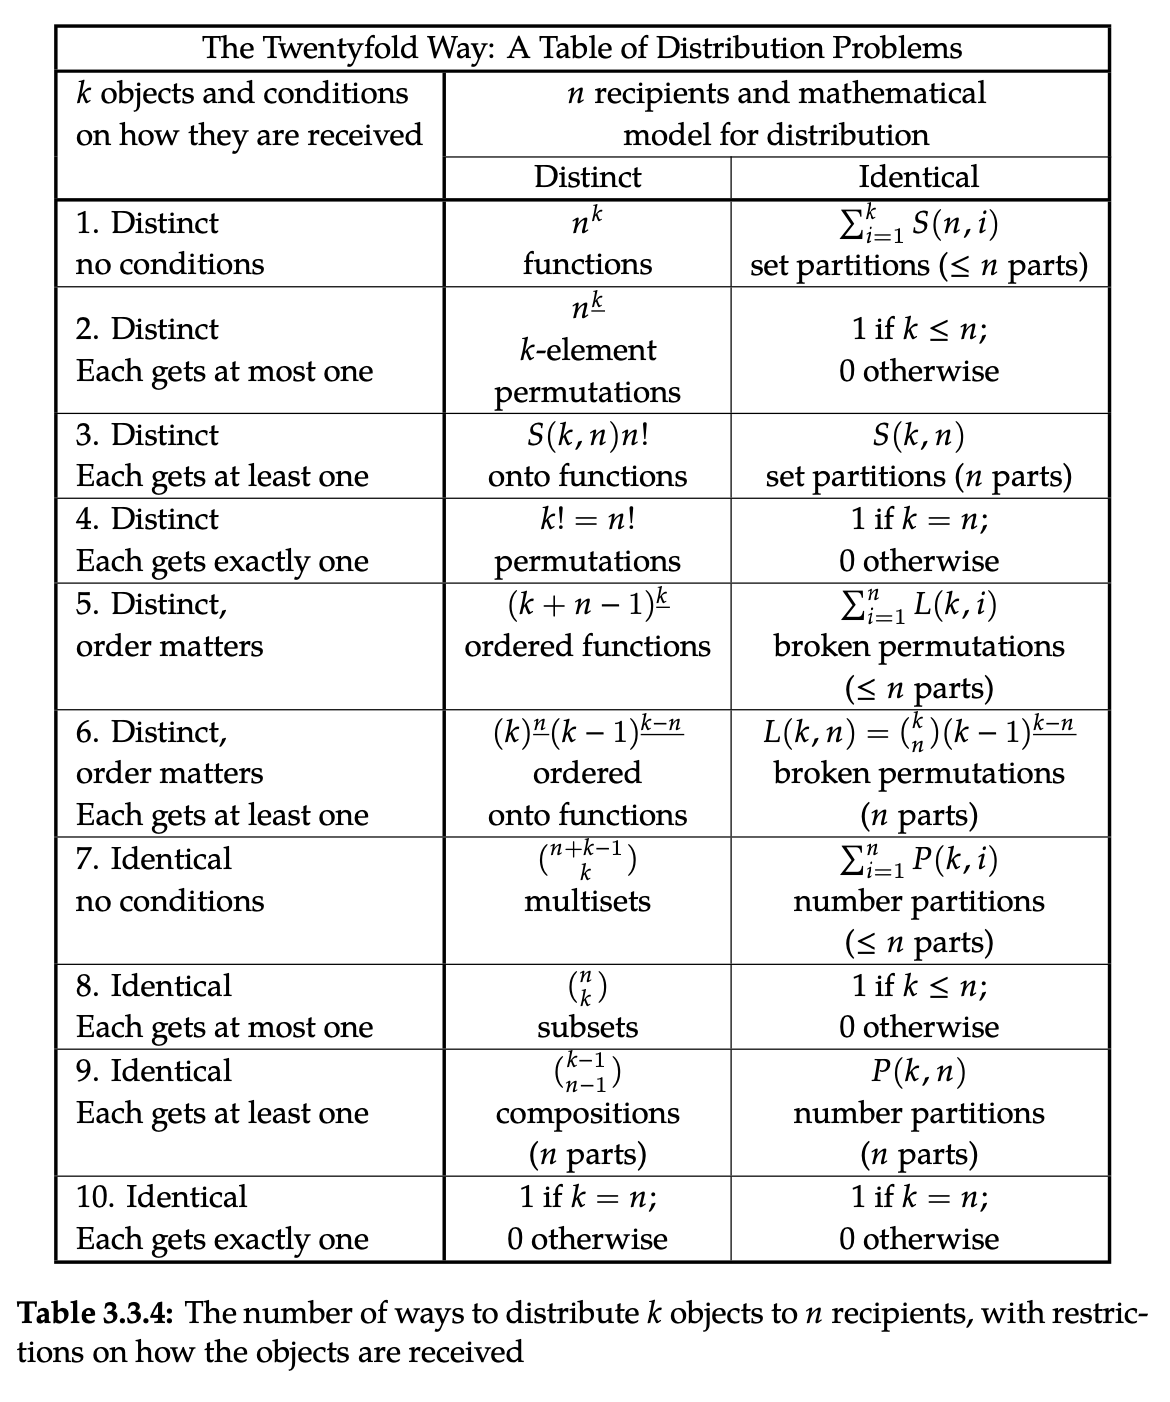
\includegraphics[width=0.5\textwidth]{twentyfoldway.png}
\end{figure}



% Distinct Objects, No Conditions
\subsection{Distinct Objects}


%% Distinct Recipients
\subsubsection{Distinct Recipients}
The $k$ objects are assigned to $n$ recipients with no conditions as to the number of objects each recipient receives. This is the same as assigning the elements of a $k$-tuple from a selection of $n$ \underline{with} replacement.

\begin{equation}	
\begin{array}{l}
S = \{ (a_1,a_2,...,a_k) | a_i \in A, |A| = n \}\\
\\
|S| = n^k
\end{array}
\end{equation}



\subparagraph{Pool Balls into Labeled Buckets} All possible ways to put $k$ pool balls, which all have different numbers and colors, into $n$ labeled buckets. Some of the buckets might be empty, and others might contain more than one of the pool balls.

\subparagraph{Functions} All possible functions $f:x \rightarrow y$ with $\{x | x\in A, |A| = k \}$ and $\{y | y\in B, |B| = n\}$.

\subparagraph{Binary Strings of Length $k$} The $k$ distinct positions of a binary string $(i_1,i_2,...,i_k)$ of length $k$ are assigned to an element of the set $A\in[0,1]$. The number of possible binary strings of length $k$ is $2^k$.

\subparagraph{Subsets of a $k$-Element Set} The subsets of a set of $k$ distinct elements are formed by assigning each of its $k$ distinguishable elements to one of the two labels $A\in [\mathrm{included},\mathrm{excluded}]$. The number of possible subsets, including the empty subset and the full set, is $2^k$.


%% Indistinct Recipients
\subsubsection{Indistinct Recipients}
The $k$ objects are assigned to a recipient that is not distinct. 

\begin{equation}
|A| = \sum_{i=1}^k S(n,i)
\end{equation}

Where $S(k,n)$ is the Stirling number of the second kind that gives the number of ways that $k$ objects can be distributed across $n$ non-empty indistinct sets. The sum above takes care of the case where the $k$ objects are divided into \underline{up to} $n$ collections.  

A closed form expression for the Stirling Numbers of the second kind is (c.f. section \ref{sec:stirling2}): 

\begin{equation}
S(k,n) = \left\{ \begin{array}{c} k \\n \end{array} \right\} = \frac{1}{n!}\sum_{j=0}^n (-1)^{n-j} {n \choose j }j^k
\label{eq:stirling2}
\end{equation}


\subparagraph{Pool Balls into Unlabeled Bags} All possible ways to put $k$ pool balls, which all have different numbers and colors, into $n$ unlabeled bags. Some of the bags might be empty, and others might contain more than one of the pool balls.


% Distinct Objects, At Most One
\subsection{Distinct Objects, Every Recipient Receives At Most One}

%% Distinct Recipients
\subsubsection{Distinct Recipients}
At most one of $k$ distinct objects are assigned to one of $n$ distinct recipients. This is the same as assigning the elements of a $k$-tuple from a selection of $n$ \underline{without} replacement, so that first there are $n$ choices, then $n-1$ choices, $n-2$, etc.

\begin{equation}	
\begin{array}{l}
S = \{ (a_1,a_2,...,a_k) | a_i \in A, |A| = n, a_i\neq a_j\}\\
\\
|S| = \frac{n!}{(n-k)!} = n^{\underline{k}}\ \ \mathrm{if\ }k\leq n,\ 0\ \mathrm{otherwise.}
\end{array}
\end{equation}

\subparagraph{At Most One Pool Ball into Labeled Buckets} All possible ways to put $k$ pool balls, which all have different numbers and colors, into $n$ labeled buckets, but the buckets can have at most one pool ball in them. In other words, you choose any $k$ out of the $n$ labeled buckets and put one pool ball into them. 

\subparagraph{One-to-One Functions} All possible functions $f:x \rightarrow y$ with $\{x | x\in A, |A| = k \}$ and $\{y | y\in B, |B| = n\}$ subject to the constraint that $f(a) = f(b)$ implies $a=b$. That is, the functions are one-to-one, or injective.

\subparagraph{k-element Permutations of $n$ elements}  Each of the $k$ positions in a $k$-element permutation are distinct objects. These are each assigned to one of $n$ possible values, where each value can only show up once. 

\subparagraph{Books on a Shelf} How many ways are there to order $k$ books on a library shelf when there are $n$ different books available. 


%% Indistinct Recipients
\subsubsection{Indistinct Recipients}
At most one of $k$ distinct objects are assigned to one of $n$ indistinct recipients. This is the same as assigning the elements of a $k$-tuple from a selection of $n$ \underline{without} replacement. Except ,since the recipients are all indistinct, there is only one type of choice of recipient for each object. Either each object finds a recipient if $k\leq n$, or it is impossible to distribute at most one object to each recipient because $n < k$.

\begin{equation}
\begin{array}{l}
S = \{ (a_1,a_2,...,a_k) | a_i \in A, |A| = n, a_i=a_j\}\\
\\
|S| = 1\ \ \mathrm{if\ }k\leq n,\ 0\ \mathrm{otherwise.}
\end{array}
\end{equation}



\subparagraph{At Most One Pool Ball into Unlabeled Bags} All possible ways to put $k$ pool balls, which all have different numbers and colors, into $n$ unlabeled bags, but the bags can have at most one pool ball in them. The bags are identical, so the only result is one where there are $k$ bags with a ball in them and $n-k$ without a ball in them. If there are not enough bags, then there is no possible result. 

\subparagraph{Distributing Candy} There are $n$ pieces of identical candy and $k$ kids. How many ways are there to give each kid a piece of candy? If there is enough candy, the answer is one. Everyone gets candy. If there is not enough candy then the answer is zero. There is no way to give everyone candy if there's not enough candy.


% Distinct Objects, At Least One
\subsection{Distinct Objects, Every Recipient Receives at Least One}

%% Distinct Recipients
\subsubsection{Distinct Recipients}

\begin{equation}
|A| = n!S(k,n) =n! \left\{ \begin{array}{c} k \\n \end{array}\right\} = n! \frac{1}{n!}\sum_{j=0}^n (-1)^{n-j} {n \choose j }j^k\end{equation}

Where $S(k,n)$	 denotes the Stirling function of the second kind.


\subparagraph{At Least One Pool Ball into Labeled Buckets} All possible ways to put $k$ pool balls, which all have different numbers and colors, into $n$ labeled buckets, so that all of the buckets have at least one ball in them. This is the same number of combinations as if the buckets were unlabeled, but multiplied with $n!$ ways of applying a label to them.

\subparagraph{Onto Functions} All possible functions $f:x \rightarrow y$ with $\{x | x\in A, |A| = k \}$ and $\{y | y\in B, |B| = n\}$ subject to the constraint that there is an element $x$ in the domain so that $f(x)=y$ for each element $y$ of the codomain. That is the functions are onto, or surjective.


%% Indistinct Recipients
\subsubsection{Indistinct Recipients}
The number of ways to divide $k$ distinct objects into $n$ non-empty subets is given by the Stirling number of the second kind (c.f. section \ref{sec:stirling2}):

\begin{equation}
|A| = S(k,n) = \left\{ \begin{array}{c} k \\n \end{array} \right\} = \frac{1}{n!}\sum_{j=0}^n (-1)^{n-j} {n \choose j }j^k	\end{equation}



\subparagraph{At Least One Pool Ball into Unlabeled Bags} All possible ways to put $k$ pool balls, which all have different numbers and colors, into $n$ unlabeled bags, so that none of the bags are empty. 


% Distinct Objects, Everyone received exactly one
\subsection{Distinct Objects, Every Recipient Receives Exactly One}

% distinct recipients
\subsubsection{Distinct Recipients}
One of $k$ distinct objects are assigned to each of $n$ distinct recipients. This is the same as assigning the elements of a $k$-tuple from a selection of $n$ \underline{without} replacement and with the requirement that all of the $n$ are selected.

\begin{equation}	
\begin{array}{l}
S = \{ (a_1,a_2,...,a_k) | a_i \in A, |A| = k = n, a_i\neq a_j\}\\
\\
|S| = n! = k!\ \ \mathrm{if\ }k=n,\ 0\ \mathrm{otherwise.}
\end{array}
\end{equation}

\subparagraph{Exactly One Pool Ball into Each Labeled Buckets} All possible ways to put $k$ pool balls, which all have different numbers and colors, into $n$ labeled buckets, that there is one pool ball in each bucket. This is the same as putting one pool ball into unlabeled buckets and multiplying by the $n!$ ways of attaching a label to the buckets. If there isn't the same amount of balls and buckets then there is no possible way for them to be matched one-for-one.

\subparagraph{Bijective Functions} All possible functions $f:x \rightarrow y$ with $\{x | x\in A, |A| = k \}$ and $\{y | y\in B, |B| = n\}$ subject to the constraints that $f(a) = f(b)$ implies $a=b$ and that there is an element $x$ in the domain so that $f(x)=y$ for each element $y$ of the codomain. That is, the functions are one-to-one and onto, of bijective.

\subparagraph{Permutations} Since each of the $k$ objects is given to a different one of the $n$ recipients, there must be as many recipients as there are objects and $k=n$. The number of ways of assigning $k$ objects to $n$ recipients is $k!=n!$.

\subparagraph{Unique Identifiers} Each of $k$ entries in a database is given one of $n=k$ unique identifiers, so that each identifier leads to an entry and each entry has an identifier. 

% indistinct recipients
\subsubsection{Indistinct Recipients}

\begin{equation}	
\begin{array}{l}
S = \{ (a_1,a_2,...,a_k) | a_i \in A, |A| = k, a_i=a_j\}\\
\\
|S| = 1\ \ \mathrm{if\ }k = n,\ 0\ \mathrm{otherwise.}
\end{array}
\end{equation}


\subparagraph{Exactly One Pool Ball into Each Unlabeled Bag} All possible ways to put $k$ pool balls, which all have different numbers and colors, into $n$ unlabeled bags, that there is one pool ball in each bag. The result is that you either have $n$ bags with $n=k$ balls in them, if the two have matching numbers, or that you either have a bag or a ball left over and there is no way to match them one-for-one.

\subparagraph{Distribute without Leftovers} $k$ students are assigned to $n$ identical textbooks. How many ways are there for each child to have a textbook so that there are no textbooks left over? 


% Distinct Objects, Ordered Groups
\subsection{Distinct Objects, Distributed in Ordered Groups}

%% Distinct Recipients
\subsubsection{Distinct Recipients}
$k$ objects are distributed to $n$ different recipients with an internal ordering, so that each recipient receives an ordered list. This is the same as creating a list of $n$ sequences that are sampled from $k$ \underline{without replacement}. 

\begin{equation}
\begin{array}{l}
S = \{ (\mathbf{a}_{\{i_1\}}  = ( a_{i_{1,1}},a_{i_{1,1}},...,a_{i_{1,l}} ),\mathbf{a}_{\{i_2\}},...,\mathbf{a}_{\{i_n\}}) | \sum^n_j |\mathbf{a}_{i_j}| = k, a_{i_{j,i}} \in A, |A| = n \} \\
\\
|S| = \frac{(k + n - 1)!}{(n-1)!} = ( k+n-1)^{\underline{k}} = k! {k+n-1 \choose k}
\end{array}
\end{equation}


\subparagraph{Books on Labeled Bookshelves} $k$ books are distributed across $n$ different bookshelves. The books may all be on the same shelf, or shelves may be empty. The ordering of the books on each of the shelves matters. This is the same as taking all the $k!$ permutations of the $k$ books and multiplying it by the way of dividing that permutation up onto $n$ shelves. 

\subparagraph{Ordered Functions}  All functions $f: x \rightarrow y$ with $\{x | x\in A, |A| = k \}$ and $\{y | y\in B, |B| = n\}$ that assign ordered sequences of elements in $x$ to elements of $y$.

%% Indistinct Recipients
\subsubsection{Indistinct Recipients}
$k$ objects are broken up into $n$ 

\begin{equation}
|S| = \sum_{i=1}^n L(k,i) 
\end{equation}

where $L(k,n)$ are the Lah numbers, which describe "How many ways can $k$ objects be distributed to $n$ recipients if order matters and each recipient receives at least 1". They are given by:

\begin{equation}
L(k,n)= {k \choose n} (k-1)^{\underline{k-n}} = \frac{k!}{n!}{ k-1 \choose n-1 }
\end{equation}

The sum considers the case where all $k$ objects are given to $i\leq n$ recipients, with the remaining recipients receiving none. Note that the expression is more complicated than simply dividing the case for indistinct recipients by $n!$, because more than one of the recipients might receive the same number of objects, in which case i.e. the distribution $[(0),(0),(1,2)]$ would be counted twice. The expression is analogous to the expression for distinct objects distributed to indistinct recipients, but where the objects did not have an internal ordering. In that case, instead of a sum over the Lah numbers, the sum is over the Stirling numbers of the second kind. 

The Lah numbers can be derived by imagining that first one of the $k$ distinct objects is distributed to the $n$ indistinct recipients, to make sure that each recipient receives at least one, and then adding the remaining objects to the first without restrictions. After the first $n$ distinct objects have been distributed to the recipients, the recipients are no longer indistinct, because they each have been labeled by the object they have already received. There are ${k \choose n}$ ways of distributing the first $n$ objects and $(k-n)!{k-n+n-1 \choose k-n}$ ways to add the $k-n$ remaining objects.

\subparagraph{Books into Unlabeled Boxes} $k$ books are stacked into up to $n$ different unlabeled boxes. Some of the boxes may be empty, and others may contain more than one book. The sequence in which the books are stacked in each box matters. If there are $n-r$ empty boxes and $r$ boxes that have at least one book in them, then there are ${k \choose r}$ ways of putting the first book in each of the boxes. Then there are $(k-r)!{k-r+r-1 \choose k-n}$ ways to stack the remaining books on top of those first books. 

\subparagraph{Broken Permutations $\leq n$ Parts} The permutations of $k$ distinct elements are ordered sequences of length $k$. If the sequence is cut up into \underline{up to} $n$ different parts of non-zero length, then what results are \textit{broken permutations}.

\subparagraph{Books into Boxes} $k$ different books are put into $n$ identical boxes. How many ways are there to pack the boxes if you keep track of the order in which the books in each box are stacked? 


% Distinct Objects, Distributed in Ordered Groups of At Least One
\subsection{Distinct Objects, Distributed in Ordered Groups of At Least One}

% Distinct Recipients
\subsubsection{Distinct Recipients}

\begin{equation}
|S| = \frac{k!}{(k-n)!}\frac{(k-1)!}{(n-1)!} = k^{\underline{n}} (k-1)^{\underline{k-n}}
\end{equation}

\subparagraph{Books on Labeled Bookshelves} $k$ books are distributed across $n$ different labeled bookshelves. There is at least one book on each shelf. This is the same as picking $n$ books to go on the shelves first, so that all of the shelves have at least one book on them, and then distributing the remainder without restrictions. There are $k^{\underline{n}}$ ways of picking the first $n$ books for each of the $n$ shelves, and $(k-n+n-1)^{\underline{k-n}}$ ways to add the remaining $k-n$ books. 

\subparagraph{Ordered Onto Functions} All functions $f: x \rightarrow y$ with $\{x | x\in A, |A| = k \}$ and $\{y | y\in B, |B| = n\}$ that assign ordered sequences of elements in $x$ to elements of $y$, where every element $y\in B$ has an assignment of at least one element.

%% Indistinct Recipients
\subsubsection{Indistinct Recipients}
$k$ elements are divided into $n$ ordered sequences of minimum length 1.

\begin{equation}
L(k,n)= {k \choose n} (k-1)^{\underline{k-n}} = \frac{k!}{n!}{ k-1 \choose n-1 }
\end{equation}
	
\subparagraph{Books into Unlabeled Boxes} $k$ books are stacked into up to $n$ different unlabeled boxes. All of the $n$ boxes have at least one book in them. The sequence in which the books are stacked in each box matters. There are ${k \choose n}$ ways of putting the first book in each of the boxes. Then there are $(k-n)!{k-n+n-1 \choose k-n}$ ways to stack the remaining $k-n$ books on top of those first books. 

\subparagraph{Broken Permutations $n$ parts} The permutations of $k$ distinct elements are ordered sequences of length $k$. If the sequence is cut up into up to $n$ different parts, then what results are \textit{broken permutations}.

\subparagraph{Books into Boxes} $k$ different books are put into $n$ identical boxes, so that there is at least one book in each box. How many ways are there to pack the boxes if you keep track of the order in which the books in each box are stacked? 


% Identical Objects
\subsection{Identical Objects}

%% Distinct Recipients
\subsubsection{Distinct Recipients}

\begin{equation}
|S| = {k+n-1 \choose k}
\end{equation}

This coefficient can be easily derives using the "Stars and Bars" concept. A short way of explaining this is as follows: picture putting all the $k$ identical objects in a line (stars). Picture having dividers (bars) to divide the $k$ objects into $n$ groups. For $n$ groups, it is necessary to use $n-1$ dividers. Empty groups result when the dividers sit right next to each other with no object in between them, or if a divider is at the end of a sequence. In total, the objects and the dividers make for a sequence in which $k+n-1$ spots are taken up by either an object or a divider. To pick a particular way of dividing the $k$ objects up, you can either pick the $n-1$ locations of the sequence in which the dividers are located, or, equivalently, the locations in which the objects are located. There are ${k+n-1\choose n-1}={k+n-1\choose k}$ to do so.  

\subparagraph{Ping Pong Balls into Labeled Buckets} $k$ identical ping pong balls are put into $n$ labeled buckets. Some of the buckets may be empty, and other buckets might have more than one ball in them.  

\subparagraph{Multisets} Multisets are sets in which identical elements might show up several times. For example $\{a,a,b,b,b\}$. They can also be described in terms of the multiplicity of their elements. For example $[a:2, b:3, c:0]$. How many multisets can be formed with $k$ different elements of $n$ different classes?

\subparagraph{Integer Sums} How many different configurations of the $n$ integers $\{ x_i\}_n$ satisfy $x_1 + x_2 + ... + x_n = k$?

\subparagraph{Bosons in Degenerate States} In how many ways might $k$ Bosons populate $n$ degenerate states?

%% Indistinct Recipients
\subsubsection{Indistinct Recipients}

\begin{equation}
|S| = \sum_{i=1}^n P(k,i)
\end{equation}

It turns out that there is no known formula for $P(k,n)$.

\subparagraph{Ping Pong Balls into Unlabeled Bags} $k$ identical ping pong balls are put into $n$ unlabeled bags. Some of the bags might be empty, and other bags might have more than one ball in them.

\subparagraph{Number Partitions} How many ways are there to divide $k$ objects across \underline{up to} $n$ piles. How many ways are there to divide an integer $k$ into a sum of $n$ integers (including zeros). For example: for $k=5$, $n=3$, the partitions are $5+0+0, 4+1+0, 3+2+0, 3+1+1, 2+2+1$.

\subparagraph{Unlabeled Multiplicities of Multisets} For multisets of $k$ elements with $n$ different classes, what is the number of possible multiplicities? For example, a multiset of $k=3$ elements from $n=2$ classes could have multiplicities $[a:3,b:0], [a:2,b:1],[a:1,b:2],[a:0,b:3]$. If we do not care about the labels $a,b$, then the ways that the the $k$ elements migth be distributed are $[3,0]$ and $[2,1]$.

\subparagraph{Boxes of Marbles} $k$ marbles are randomly put into $n$ boxes. How many ways are there for the weight to be distributed among the boxes?



% Identical Objects, Each gets at most one
\subsection{Identical Objects, Each Receives At Most One}

%% Distinct Recipients
\subsubsection{Distinct Recipients}
$k$ identical objects are distributed across $n$ recipients so that each recipient recieves at most one. That amounts to choosing $k$ out of the $n$ recipients who will receive an object.

\begin{equation}
|S| = { n \choose k}
\end{equation}


\subparagraph{At Most One Ping Pong Balls into Labeled Buckets} $k$ identical ping pong balls are distributed across $n$ different buckets, so that $k$ buckets have one ball in them and $n-k$ buckets are empty. This is the same as choosing $k$ out of the $n$ buckets, for which there are $n\times(n-1)\times(n-2)\times\hdots\times(n-k+1)$ choices for the $k$ balls, and correcting for the internal orderings of the $k$ balls by dividing by $k!$ because the balls are identical.

\subparagraph{Subsets} $k$ element subsets of a set of size $n$. The subsets are formed by either choosing the $k$ elements that are included or the $n-k$ elements that are excluded.

\subparagraph{Set Binary Labels} The problem can also be thought of as assigning a binary label to $n$ elements, where there are $k$ times $1$ and $n-k$ times 0.

%% Indistinct Recipients
\subsubsection{Indistinct Recipients}

\begin{equation}
|S| = 1\ \ \mathrm{if\ }k \leq n,\ 0\ \mathrm{otherwise}
\end{equation}

\subparagraph{At Most One Ping Pong Ball into Unlabeled Bags}  $k$ identical ping pong balls are put into $n$ identical bags. The result is either $k$ bags with ping pong balls and $n-k$ empty bags, or there is no possible result if there are not enough bags (i.e. if $k>n$).

\subparagraph{Boxes} How many ways are there to put $k$ marbles in $n$ boxes, if each box is only big enough for one marble. One, if there are enough boxes, or zero, if there aren't enough boxes.


% Identical Everyone Gets At Least one
\subsection{Identical Objects, Each Receives At Least One}

%% Distinct Recipients
\subsubsection{Distinct Recipients}
This problem is the same as giving each of $n$ recipients one of $k$ objects, and then distributing the remaining $k-n$ objects arbitrarily.  

\begin{equation}
|S| = {k+n-1-k \choose k-n}= {n-1 \choose k-1}
\end{equation}

This can be derived by picturing first distributing one object to each of the $n$ recipients, ensuring that each recipient has at least one, and then distributing the remaining $k-n$ objects arbitrarily. There is only one way to give each recipient one of the identical objects, and then there are ${k-n+n-1\choose k-n}$ ways to distribute the remaining $k-n$ objects arbitrarily across the recipients.

\subparagraph{At Least One Ping Pong Ball into Labeled Buckets} $k$ ping pong balls are distributed into $n$ labeled buckets so that there is at least one ping pong ball in each bucket. The labeled buckets may have more than one ping pong ball in them.

\subparagraph{Compositions $n$ Parts} How many ways are there to assign $k$ identical objects to $n$ labeled sets of at least one object?

% Indistinct Recipients
\subsubsection{Indistinct Recipients}

\begin{equation}
|S| = P(k,n)
\end{equation}

It turns out that there is no known formula for $P(k,n)$.

\subparagraph{At Least One Ping Pong Ball in Unlabeled Bags} $k$ identical ping pong balls are distributed across $n$ unlabeled bags, so that none of the bags are empty. 

\subparagraph{Partitions in $n$ Parts} How many ways are there to make $n$ piles from $k$ objects.



% Identical Each Gets Exactly one
\subsection{Identical Objects, Each Receives Exactly One}

%% Distinct Recipients 
\subsubsection{Distinct Recipients}

\begin{equation}
|S| = 1\ \ \mathrm{if\ }k = n,\ 0\ \mathrm{otherwise}
\end{equation}  

\subparagraph{One Ping Pong Ball into Each Labeled Bucket} $k$ identical ping pong balls are distributed across $n$ labeled buckets so that each bucket has one ping pong ball in it. If $k=n$, then there is one way to put one ball in each bucket. If the numbers do not match up, then there is no way to match them one-for-one.

%% Indistinct Recipients
\subsubsection{Indistinct Recipients}

\begin{equation}
|S| = 1\ \ \mathrm{if\ }k = n,\ 0\ \mathrm{otherwise}
\end{equation}  

\subparagraph{One Ping Pong Ball into Each Unlabeled Bag} $k$ identical ping pong balls are distributed across $n$ identical bags so that each bags has one ping pong ball in it. If $k=n$, then there is one way to put one ball in each bag. If the numbers do not match up, then there is no way to match them one-for-one.




